\subsection{Ephemeral and Persistent Transport Clients}

These experiments performs requests sequentially with transport-layer protocols in two different ways. While the ephemeral experiment always creates a new client for each request, the persistent experiment creates only one client that performs all requests. Consequently, client creation and connection establishment overhead can be observed.

\subsection{Latency \& Throughput}

Charts on Figures \ref{fig:persistent_transport_latency}, \ref{fig:ephemeral_transport_latency}, \ref{fig:parallel_transport_latency}, \ref{fig:persistent_transport_throughput}, \ref{fig:ephemeral_transport_throughput}, \ref{fig:parallel_transport_throughput} represent the \gls{p90} of Latency and Throughput of all 10000 requests made by the persistent and ephemeral clients during the experiments.

Throughout these charts it is possible to observe an order pattern. Local experiments usually were more performatic when compared to Single-\gls{az} experiments. Additionally, the latter results were better than Multi-\gls{az} experiments due to the overhead from sending the datagram to another data center, even though remaining in the same region.

\gls{udp} Multi-\gls{az} and Single-\gls{az} experiments only succeeded on the first two iterations of each run when the data transferred was 2KiB and 8KiB. This was expected since pure \gls{udp} does not have any reliability and is expected to lose user datagrams along the way. As was stated before, no additional logic was added to \gls{udp} since this would interfere with the results because it would alter \gls{udp} natural behaviour.

Local \gls{tcp} experiment was by far the most efficient, with almost zero latency when connection was persistent, reaching approximately 19Gb/s of speed when transferring 512KiB of data per request. It outperformed \gls{udp}, that even though is considered faster due to its unreliability and connectionless characteristics, it only reached 2.8Gb/s in the same scenario. This happened because, while \gls{tcp} is stream oriented, which enables it to send a continuous stream of data with no overhead, \gls{udp} is message oriented.

Nonetheless, ephemeral clients demonstrated that establishing connections can have a significant impact on \gls{tcp}’s performance. Local \gls{tcp} latency went from 0.19ms to 1.79ms and throughput from 19Gb/s to 2.2Gb/s. Both results are still better than other \gls{tcp} and all \gls{tcp}+\gls{tls}’ experiments \gls{p90}, but brings them to a similar level.

It is possible to observe \gls{tls} encryption overhead on \gls{tcp} during persistent clients experiments. Furthermore, during ephemeral clients this overhead increases due to having to perform a \gls{tls} handshake before every request.

QUIC’s experiments were the worst, with almost 7 times slower than \gls{tcp}+\gls{tls}’ Multi-\gls{az} experiment (with persistent client) latency and throughput. This demonstrates \gls{tcp}+\gls{tls} performs better than QUIC on a reliable network, with a low packet loss rate. However, QUIC performs better than \gls{tcp}+\gls{tls} on an unreliable network.

QUIC’s specifically designed to be used in environments such as a wireless network or a mobile device, both which have a high tendency to lose packets, and to break \gls{tcp} connections. QUIC solves these problems by implementing a more efficient way to deal with retransmission of lost packets, improving its throughput, and having a 0-\gls{rtt} handshake, which deals with broken connections by removing the need to perform a \gls{tcp} and \gls{tls} handshake.

Consequently, QUIC’s results show it's not meant to be used on distributed systems. These environments are usually part of a reliable network, meaning that \gls{tcp} is usually a better fit.

\subsection{Parallel}

All previous experiments performed requests sequentially, undermining the possible gain in efficiency of protocols that contain improvements to concurrent requests. Therefore this experiment tries to explore this scenario by performing all 10000 requests with 100 Goroutines, each performing 100 requests.

However, when packet size is the same, we fallback to a scenario where multiplexing is useless since any request performed in sequence is going to take more than the previous to complete. Therefore, this is similar to a pipelining scenario, where the requests finish in the order they were made.

\begin{figure}[h]
    \centering
    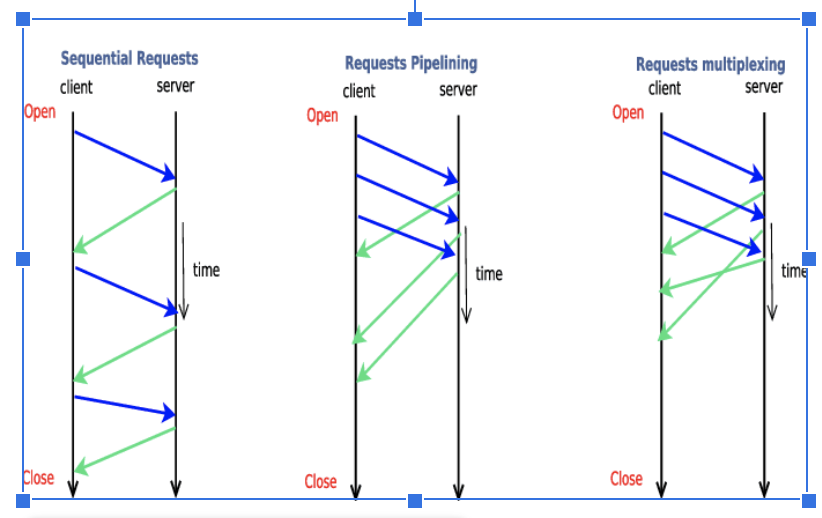
\includegraphics[width=\linewidth]{figures/pipelining.png}
    \caption{Pipelining}
    \label{fig:pipelining}
\end{figure}

\clearpage

\begin{figure}[h!]
    \centering
    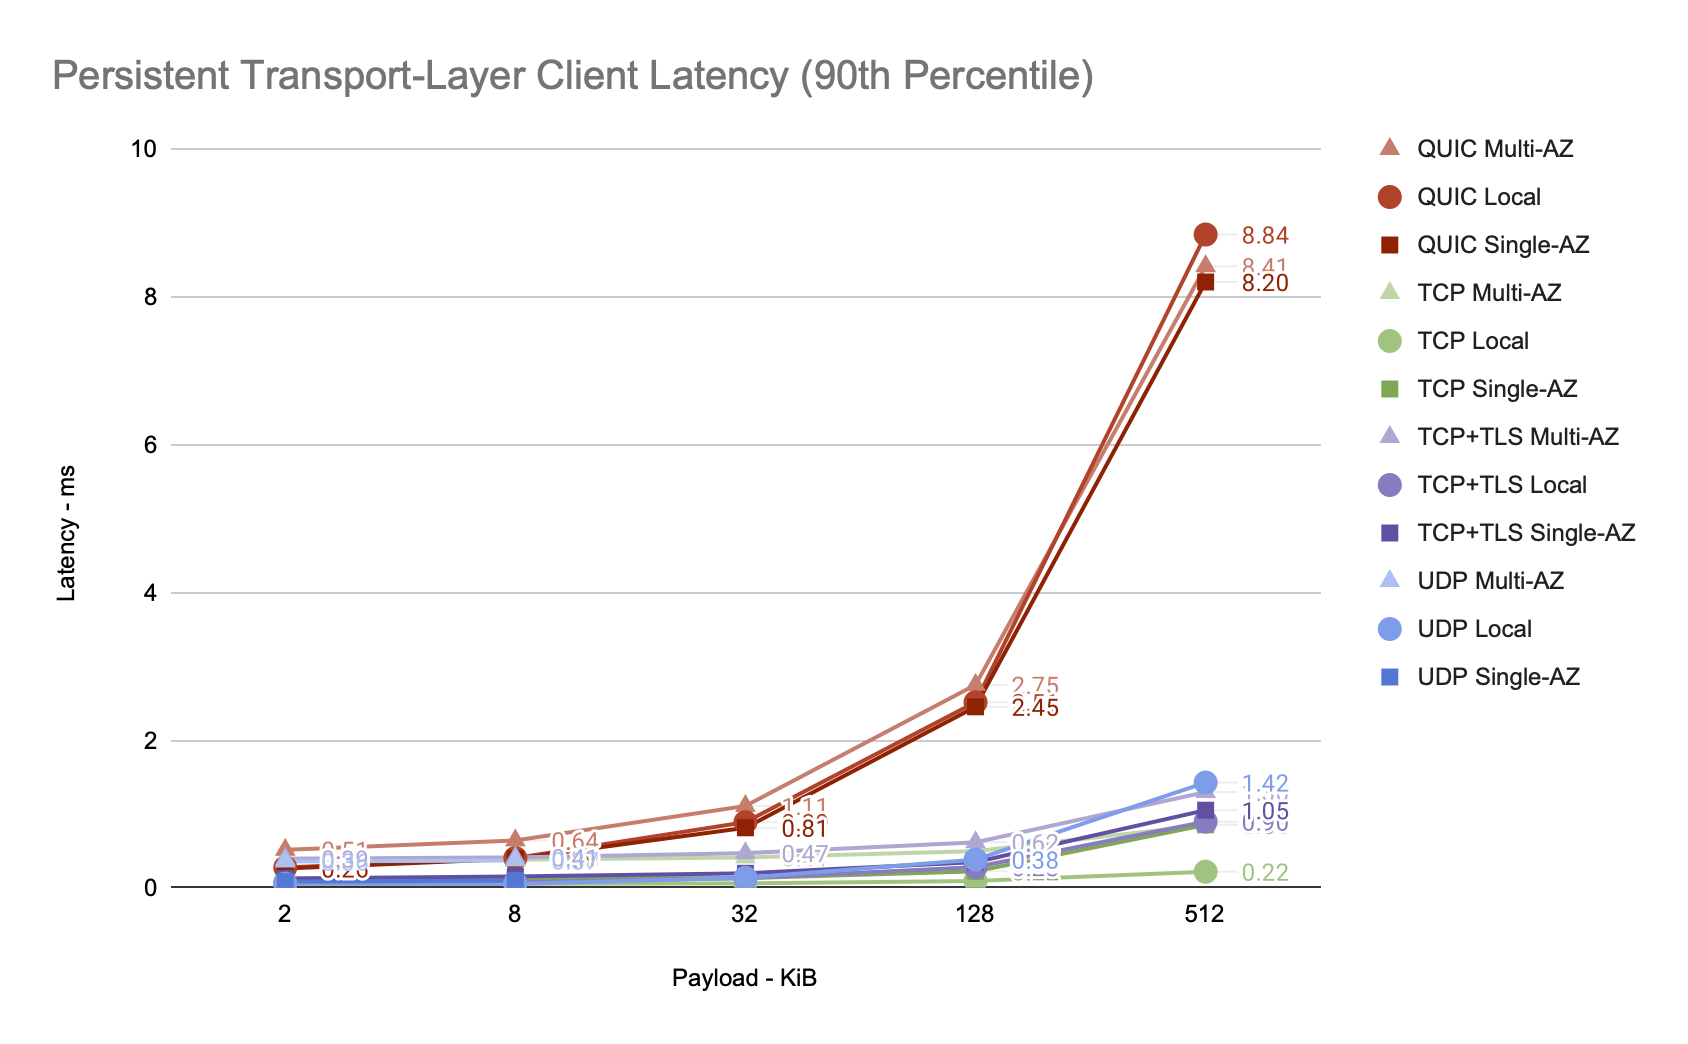
\includegraphics[width=\linewidth]{figures/charts/Persistent Transport-Layer Client Latency (90th Percentile).png}
    \caption{Persistent Transport-Layer Client Latency (90th Percentile)}
    \label{fig:persistent_transport_latency}
\end{figure}

\begin{figure}[h!]
    \centering
    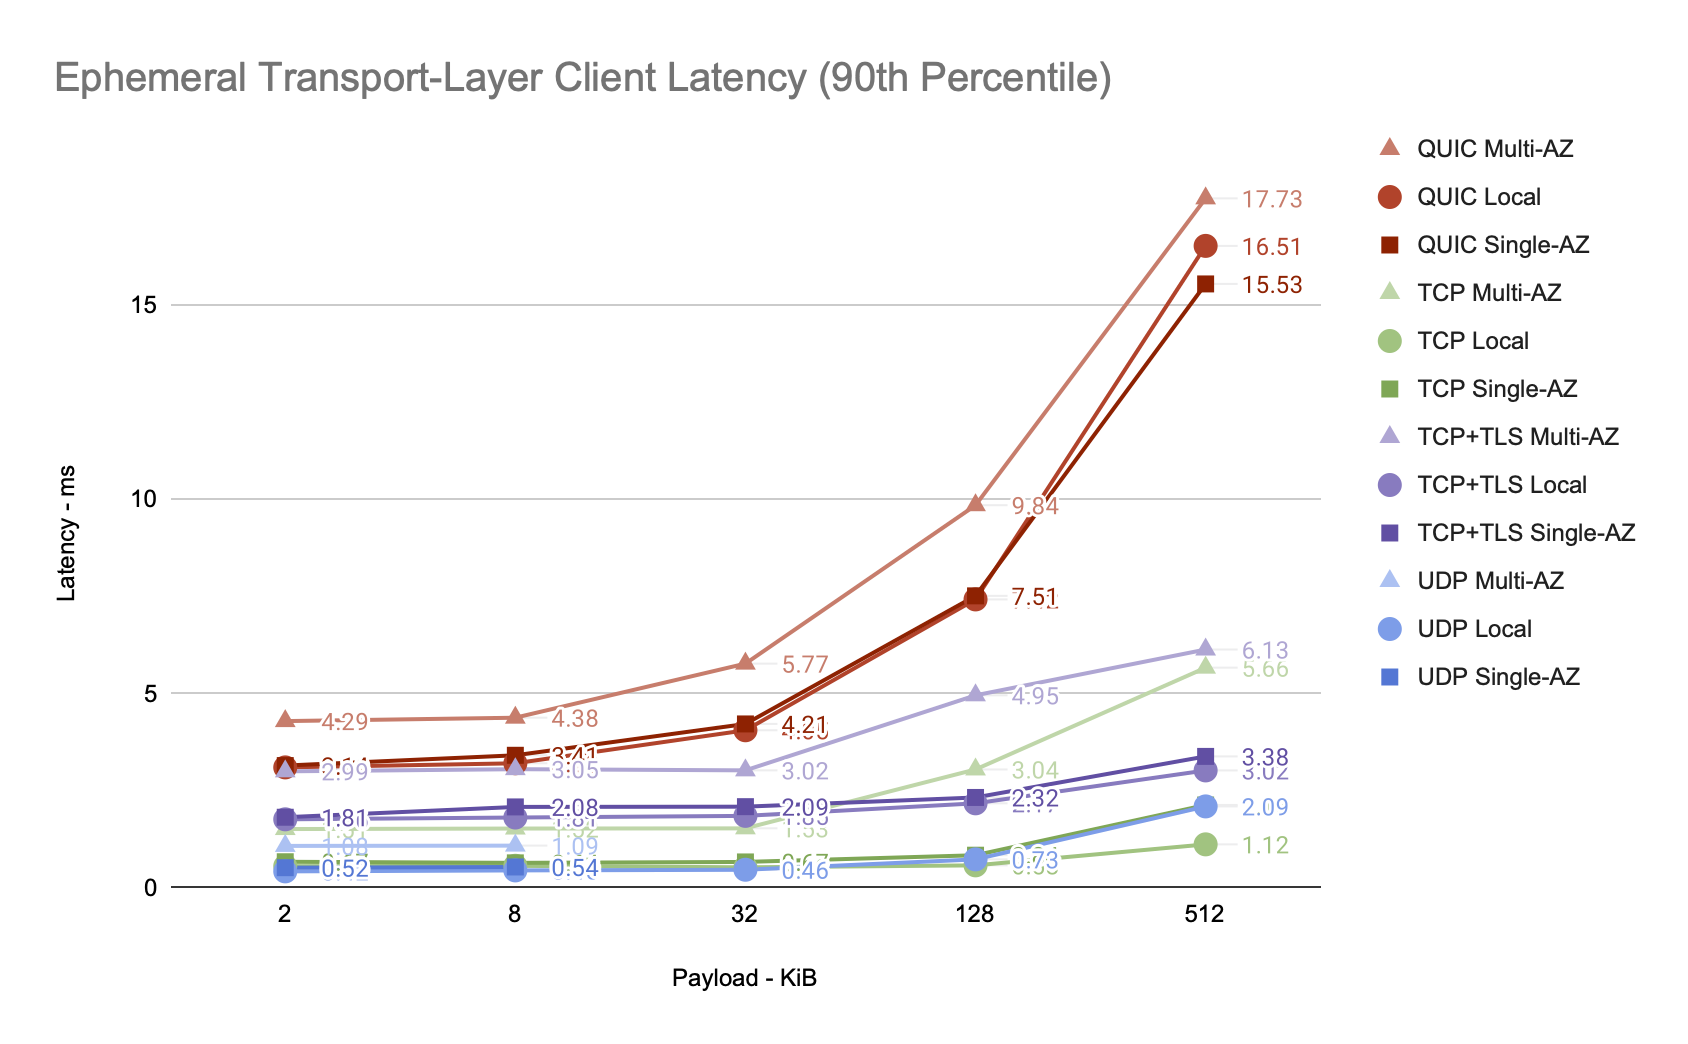
\includegraphics[width=\linewidth]{figures/charts/Ephemeral Transport-Layer Client Latency (90th Percentile).png}
    \caption{Ephemeral Transport-Layer Client Latency (90th Percentile)}
    \label{fig:ephemeral_transport_latency}
\end{figure}

\begin{figure}[h!]
    \centering
    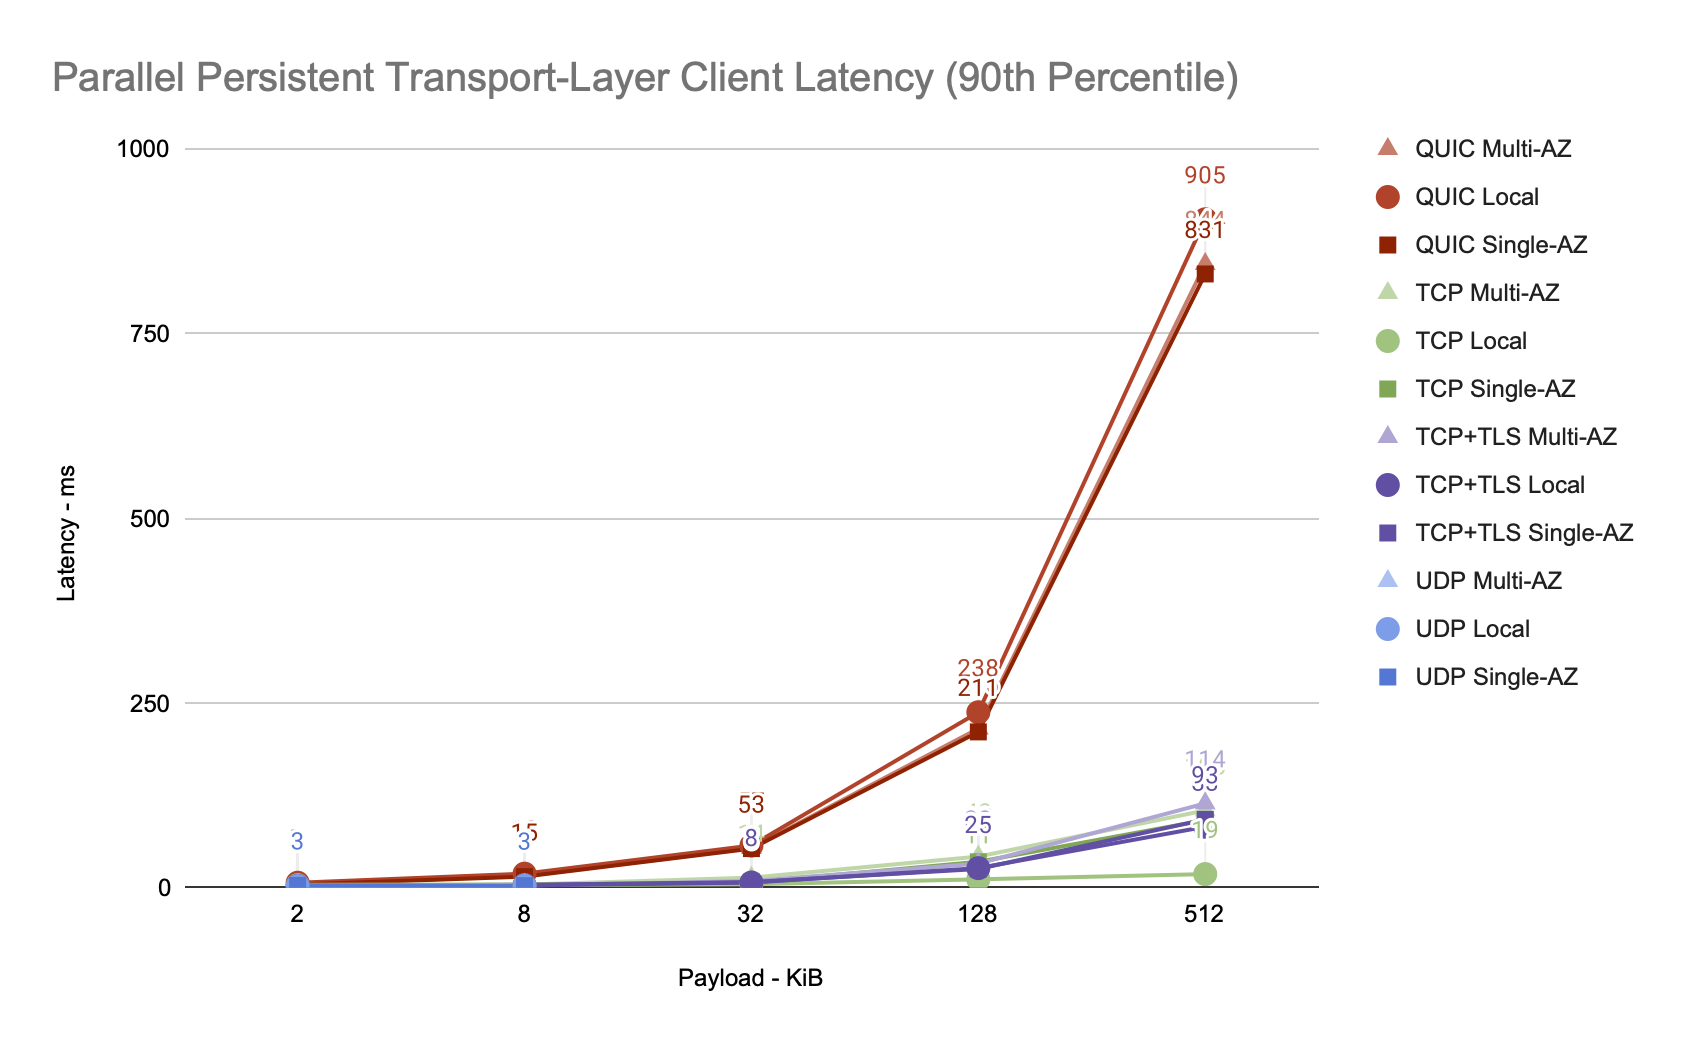
\includegraphics[width=\linewidth]{figures/charts/Parallel Persistent Transport-Layer Client Latency (90th Percentile).png}
    \caption{Parallel Persistent Transport-Layer Client Latency (90th Percentile)}
    \label{fig:parallel_transport_latency}
\end{figure}

\begin{figure}[h!]
    \centering
    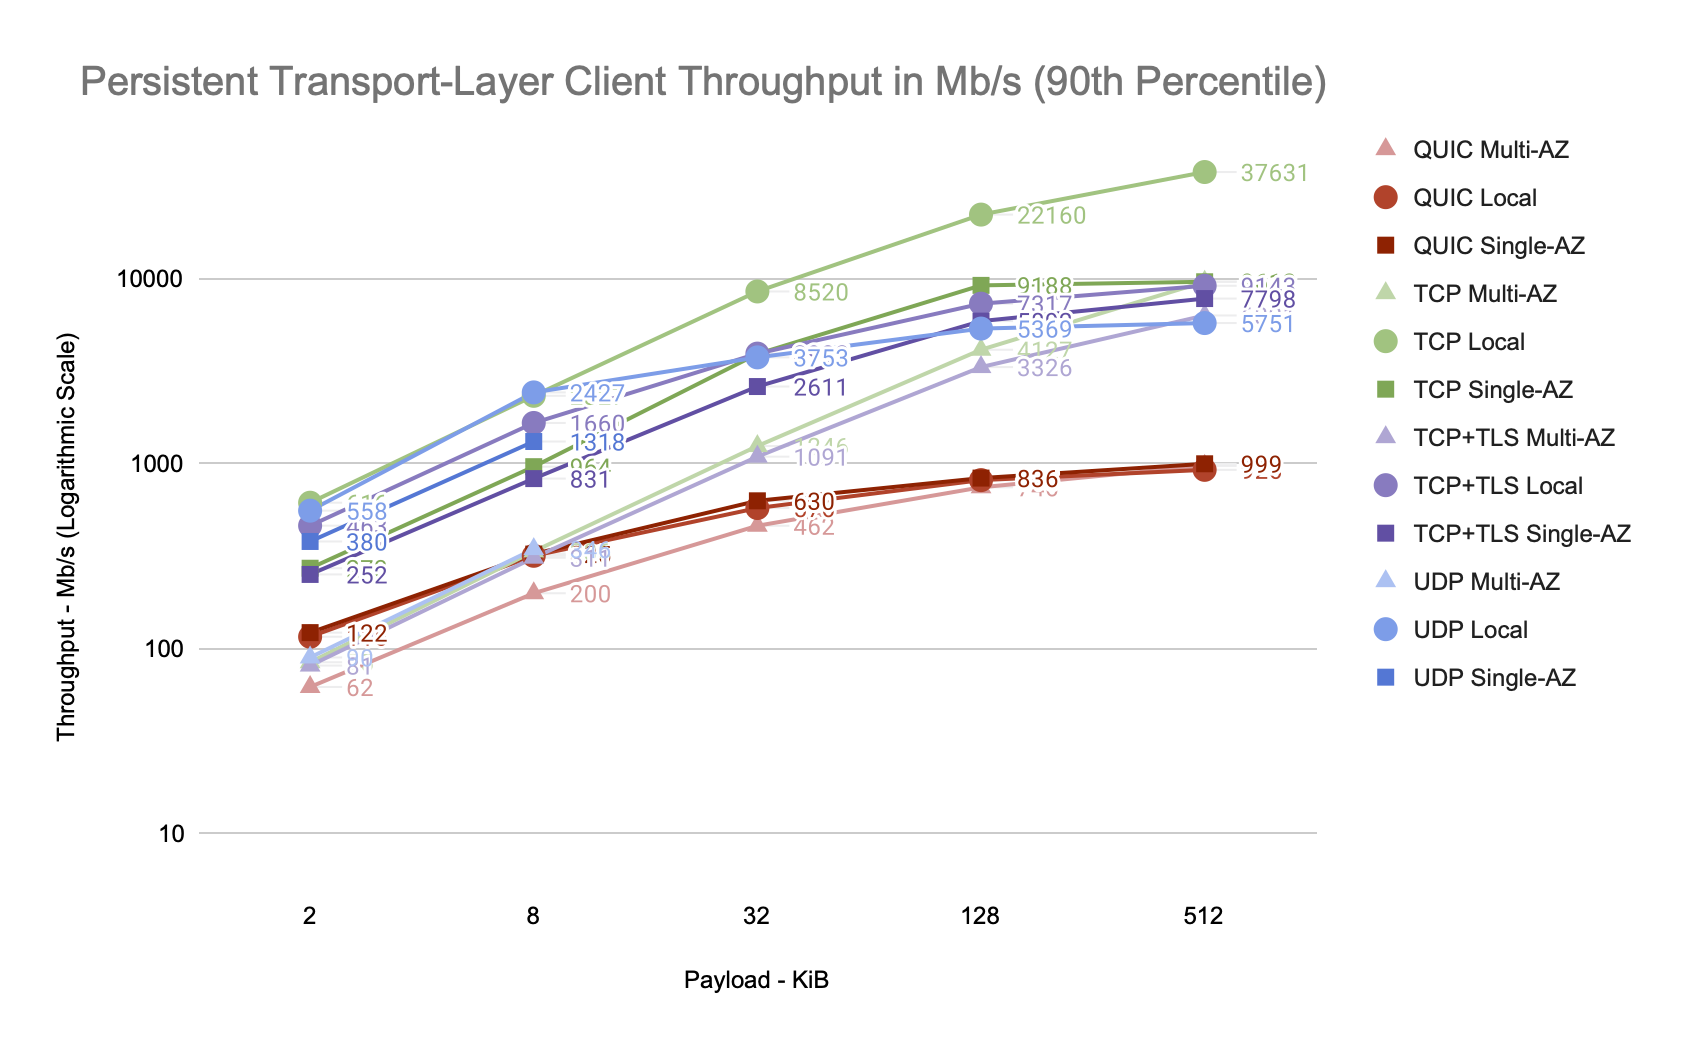
\includegraphics[width=\linewidth]{figures/charts/Persistent Transport-Layer Client Throughput in Mb_s (90th Percentile).png}
    \caption{Persistent Transport-Layer Client Throughput in Mb/s (90th Percentile)}
    \label{fig:persistent_transport_throughput}
\end{figure}

\begin{figure}[h!]
    \centering
    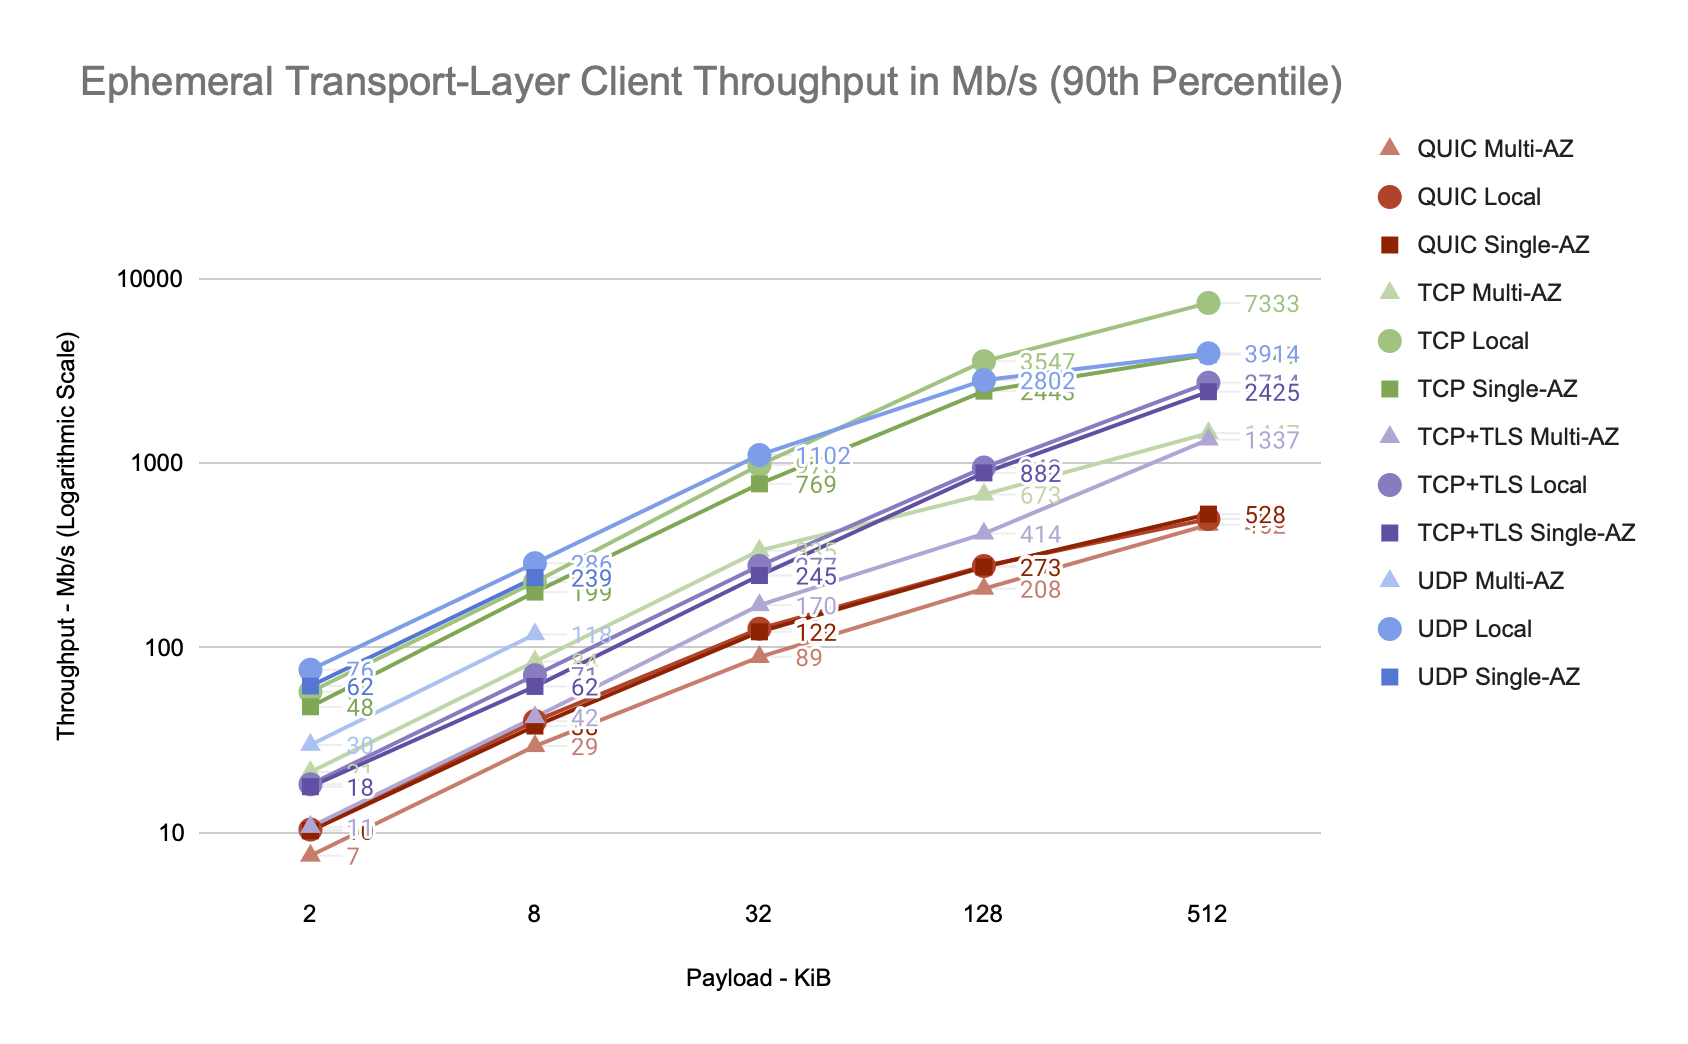
\includegraphics[width=\linewidth]{figures/charts/Ephemeral Transport-Layer Client Throughput in Mb_s (90th Percentile).png}
    \caption{Ephemeral Transport-Layer Client Throughput in Mb/s (90th Percentile)}
    \label{fig:ephemeral_transport_throughput}
\end{figure}

\begin{figure}[h!]
    \centering
    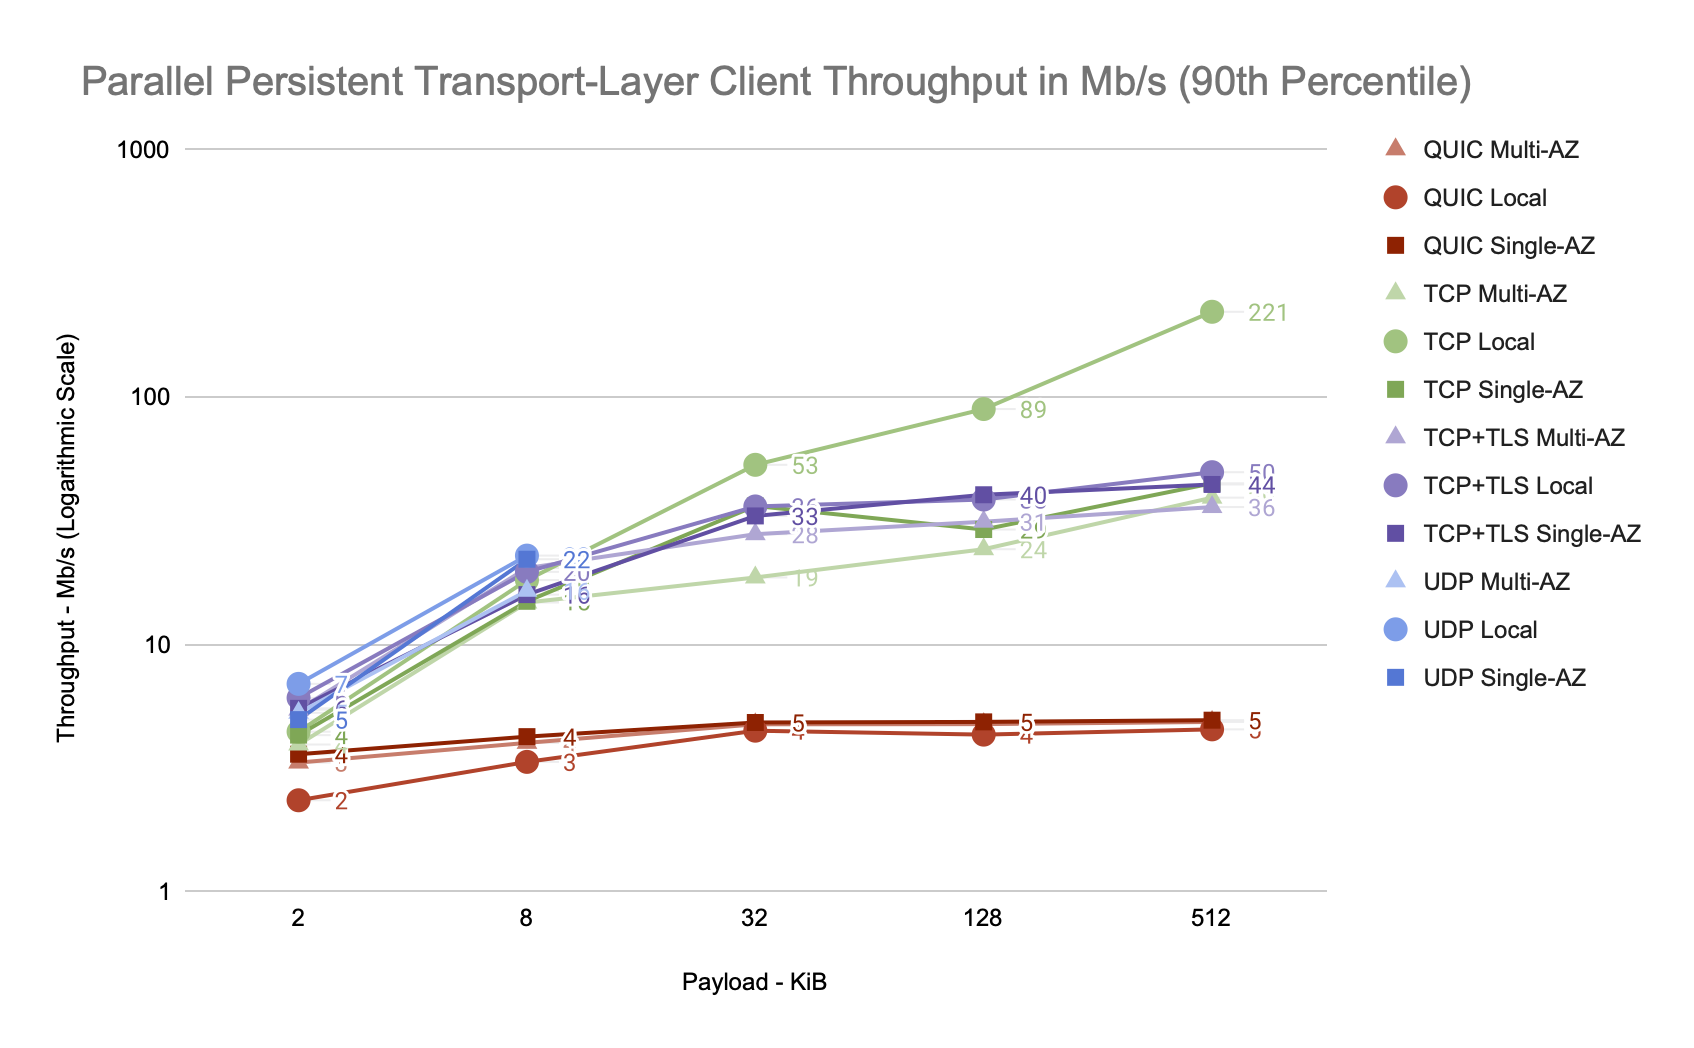
\includegraphics[width=\linewidth]{figures/charts/Parallel Persistent Transport-Layer Client Throughput in Mb_s (90th Percentile).png}
    \caption{Ephemeral Transport-Layer Client Throughput in Mb/s (90th Percentile)}
    \label{fig:parallel_transport_throughput}
\end{figure}

\clearpage

\subsubsection{CPU Usage}

Charts on Figures \ref{fig:sequential_client_app_cpu}, \ref{fig:parallel_client_app_cpu}, \ref{fig:sequential_server_app_cpu}, and \ref{fig:parallel_server_app_cpu} represent the \gls{cpu} usage of clients and servers during ephemeral and persistent experiments.

\subsubsection*{Overall Clients CPU Usage}

Application-layer protocols CPU Usage results behavior is similar to transport-layer's. Parallel requests with 32KiB and smaller payloads had a lower CPU usage when compared to sequential requests. And as requests payloads reaches 128KiB size, parallel requests CPU usage surpasses sequential requests.

\subsubsection*{HTTP/3's CPU Usage}

QUIC's CPU Usage (Figure \ref{fig:parallel_client_transport_cpu}) is almost the same as HTTP/3's (Figure \ref{fig:parallel_client_app_cpu}). As QUIC performs shift features that were usually implemented in the application-layer, it does most of the work necessary to manage traffic. Therefore, HTTP/3 is only an interface so applications can still use it as any other HTTP protocol.

\subsubsection*{Overall Server CPU Usage}

As other experiments, Server CPU usage remained roughly the same as client CPU usage. Client and servers still need to process the same amount of requests and responses, which explains why their CPU usage is so similar.

\clearpage

\begin{figure}[h!]
    \centering
    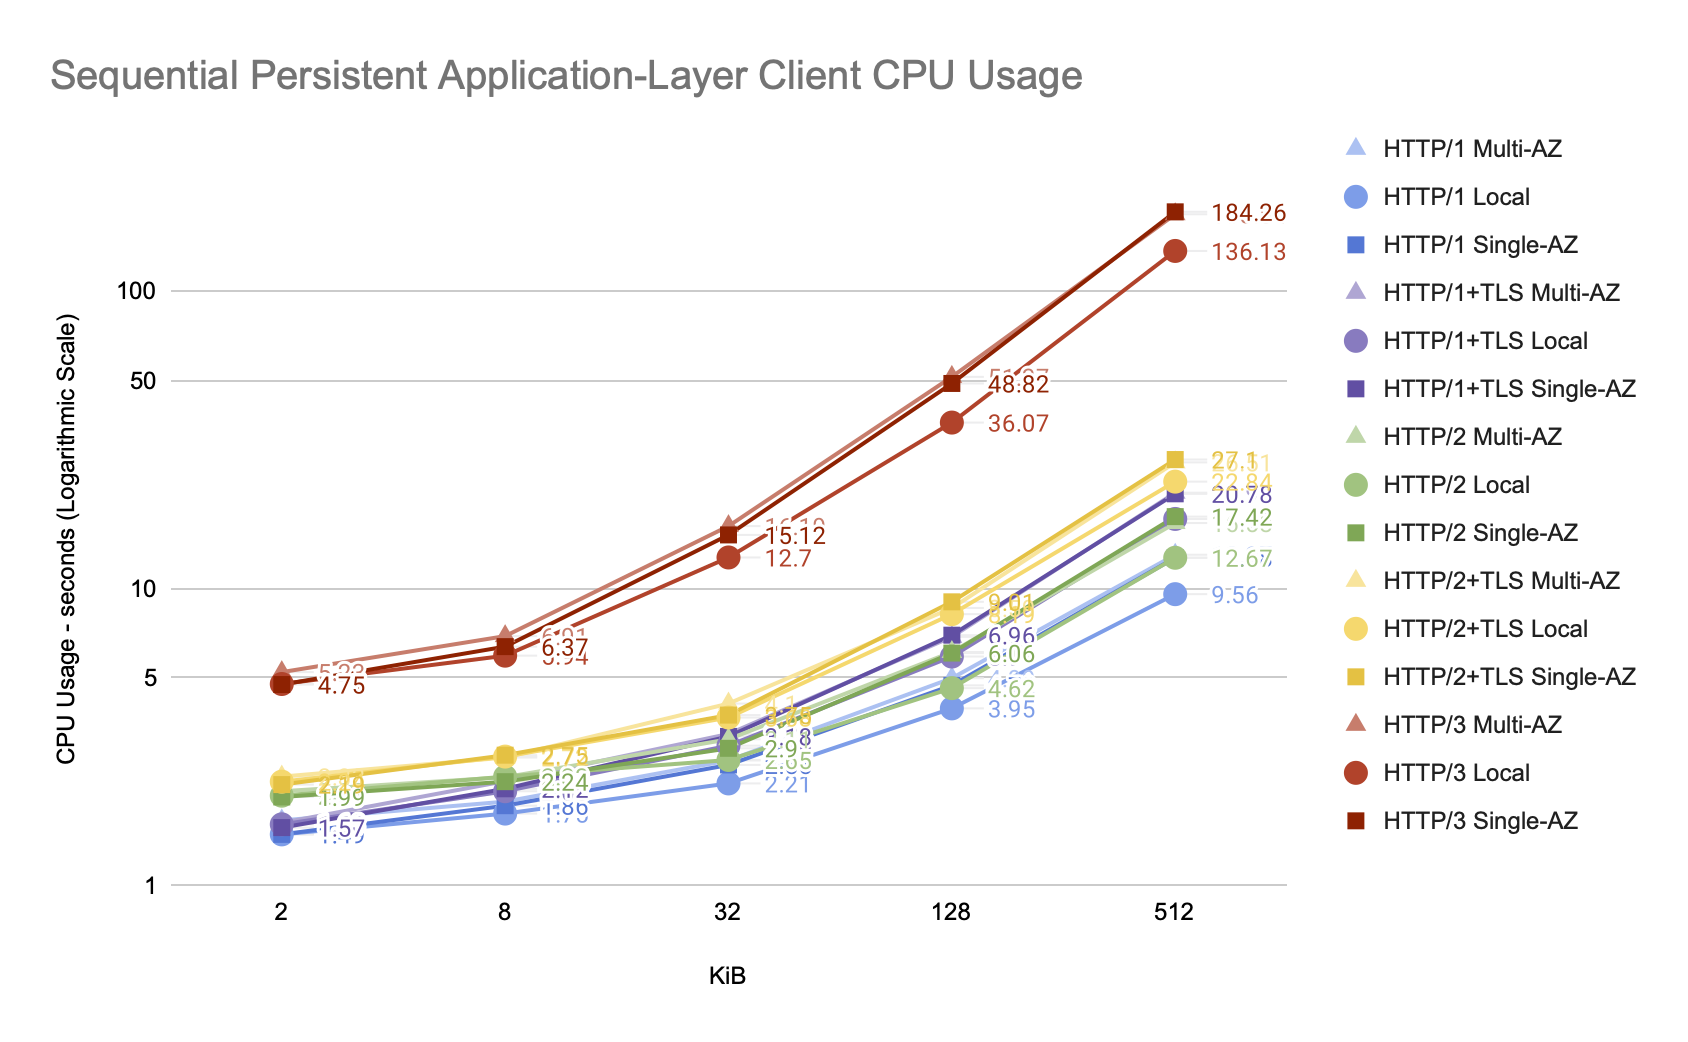
\includegraphics[width=\linewidth]{figures/charts/Sequential Persistent Application-Layer Client CPU Usage.png}
    \caption{Sequential Persistent Application-Layer Client CPU Usage}
    \label{fig:sequential_client_app_cpu}
\end{figure}
\begin{figure}[h!]
    \centering
    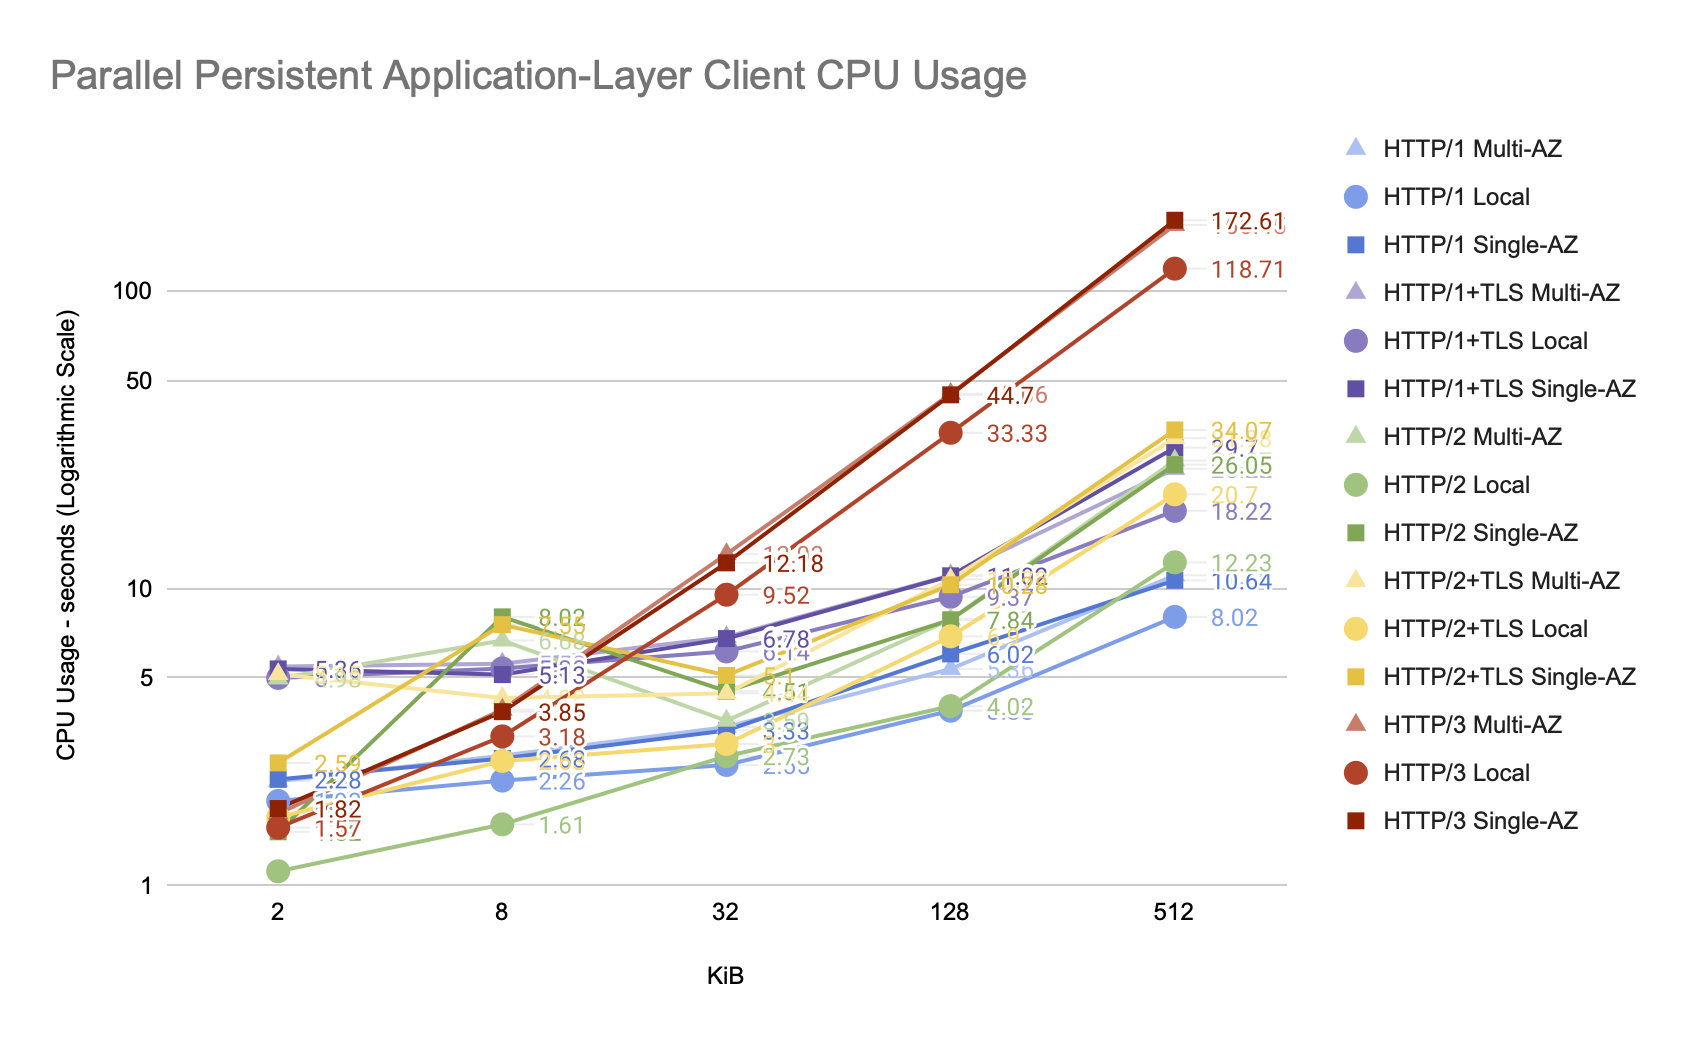
\includegraphics[width=\linewidth]{figures/charts/Parallel Persistent Application-Layer Client CPU Usage.png}
    \caption{Parallel Persistent Application-Layer Client CPU Usage}
    \label{fig:parallel_client_app_cpu}
\end{figure}

\begin{figure}[h!]
    \centering
    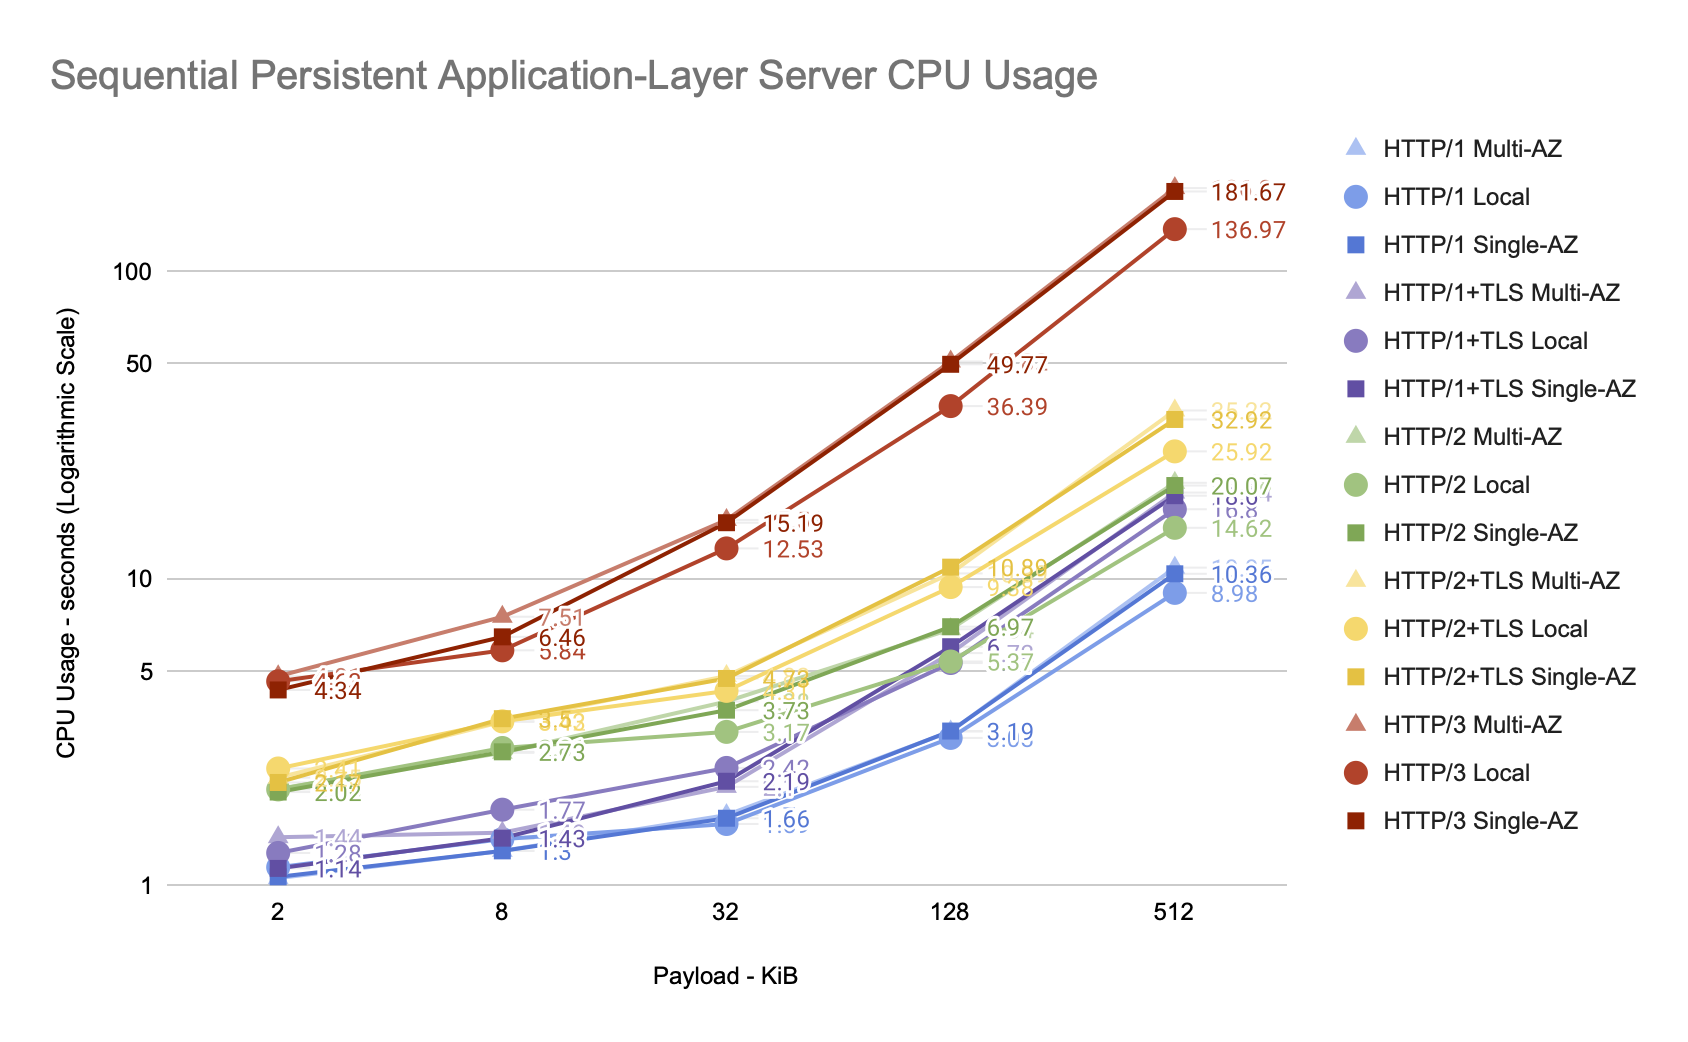
\includegraphics[width=\linewidth]{figures/charts/Sequential Persistent Application-Layer Server CPU Usage.png}
    \caption{Sequential Persistent Application-Layer Server CPU Usage}
    \label{fig:sequential_server_app_cpu}
\end{figure}
\begin{figure}[h!]
    \centering
    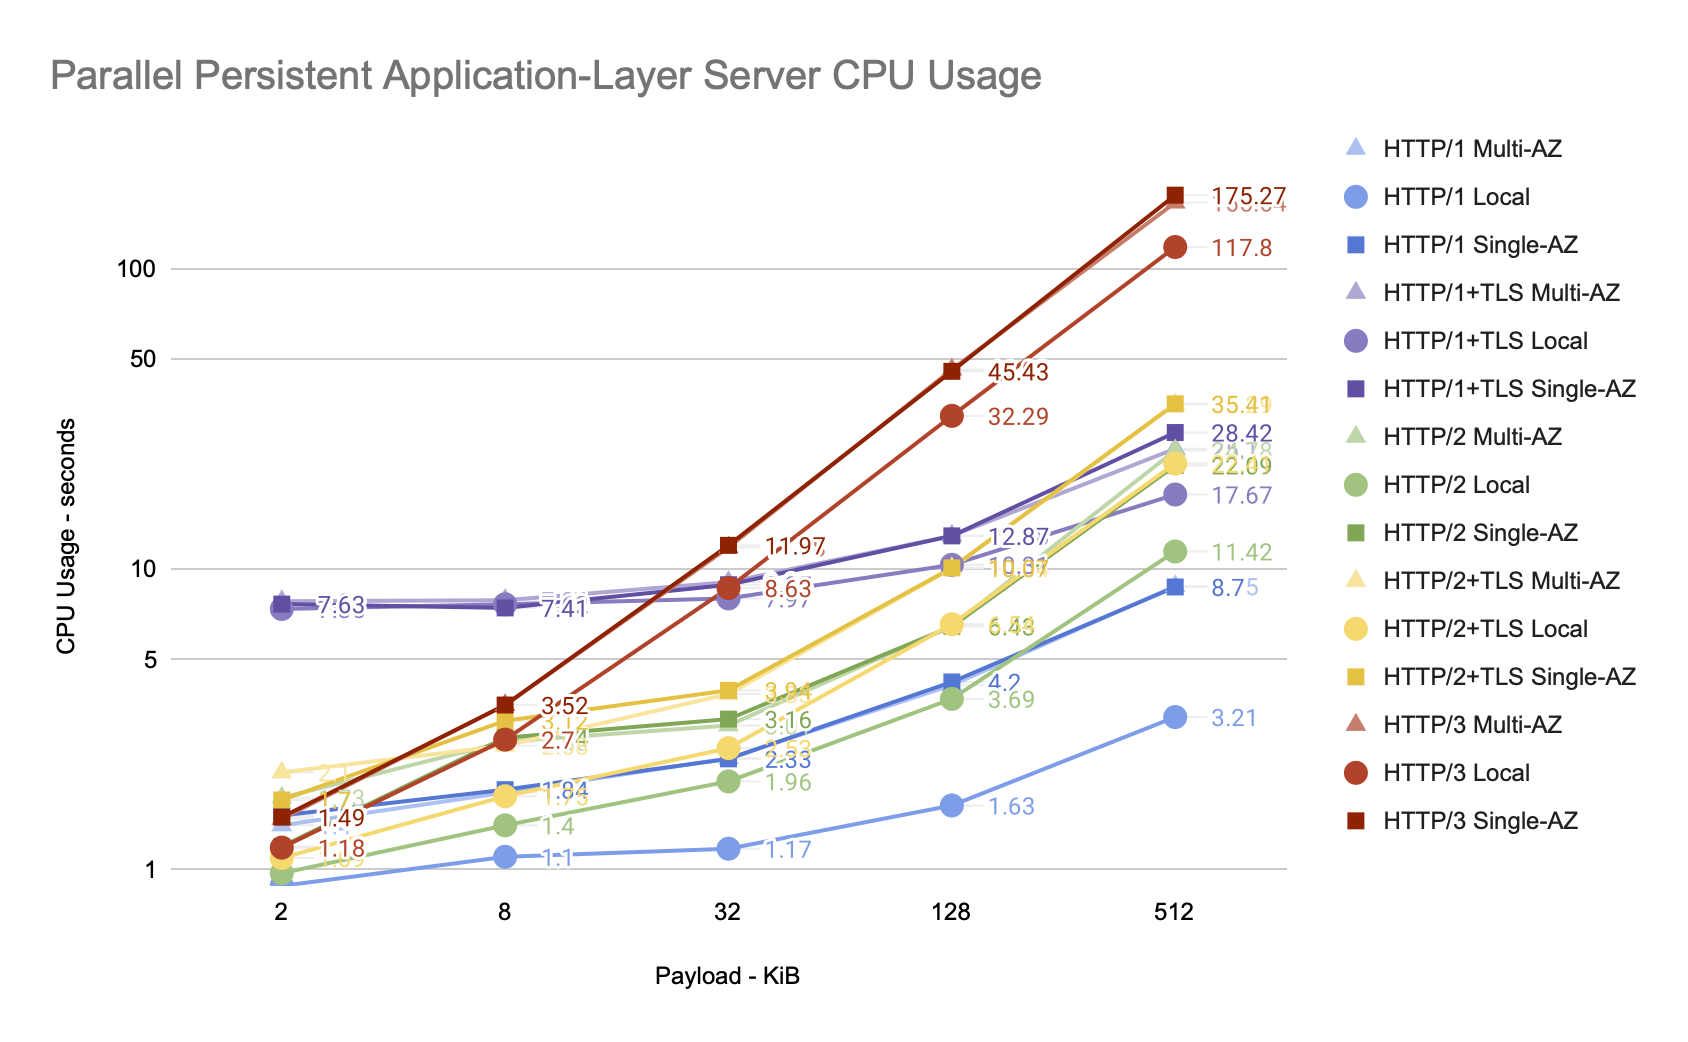
\includegraphics[width=\linewidth]{figures/charts/Parallel Persistent Application-Layer Server CPU Usage.png}
    \caption{Parallel Persistent Application-Layer Server CPU Usage}
    \label{fig:parallel_server_app_cpu}
\end{figure}

\clearpage

\subsection{Memory}

These charts represent the memory usage of clients and servers during ephemeral and persistent experiments.

These results were very similar to transport-layer experiments. \gls{http}/1 and \gls{http}/2 were the most memory efficient due to their simplicity and use of \gls{tcp} as transport protocol, which had similar results. \gls{http}/1+\gls{tls} and \gls{http}/2+\gls{tls} had increased memory usage due to \gls{tls} requirements for data encryption and \gls{tls} handshake. Finally, \gls{http}/3 had to use more memory due to QUIC’s overhead, which trades memory for efficiency.

During ephemeral experiments, Go’s garbage collector also had problems dealing with the high rate of created clients. Problem that begins worse with small data sizes, but it gets amortized as data sizes gets larger, which results in slower responses from the server, allowing Go’s garbage collector time to do its job.

\clearpage

\begin{figure}[h!]
    \centering
    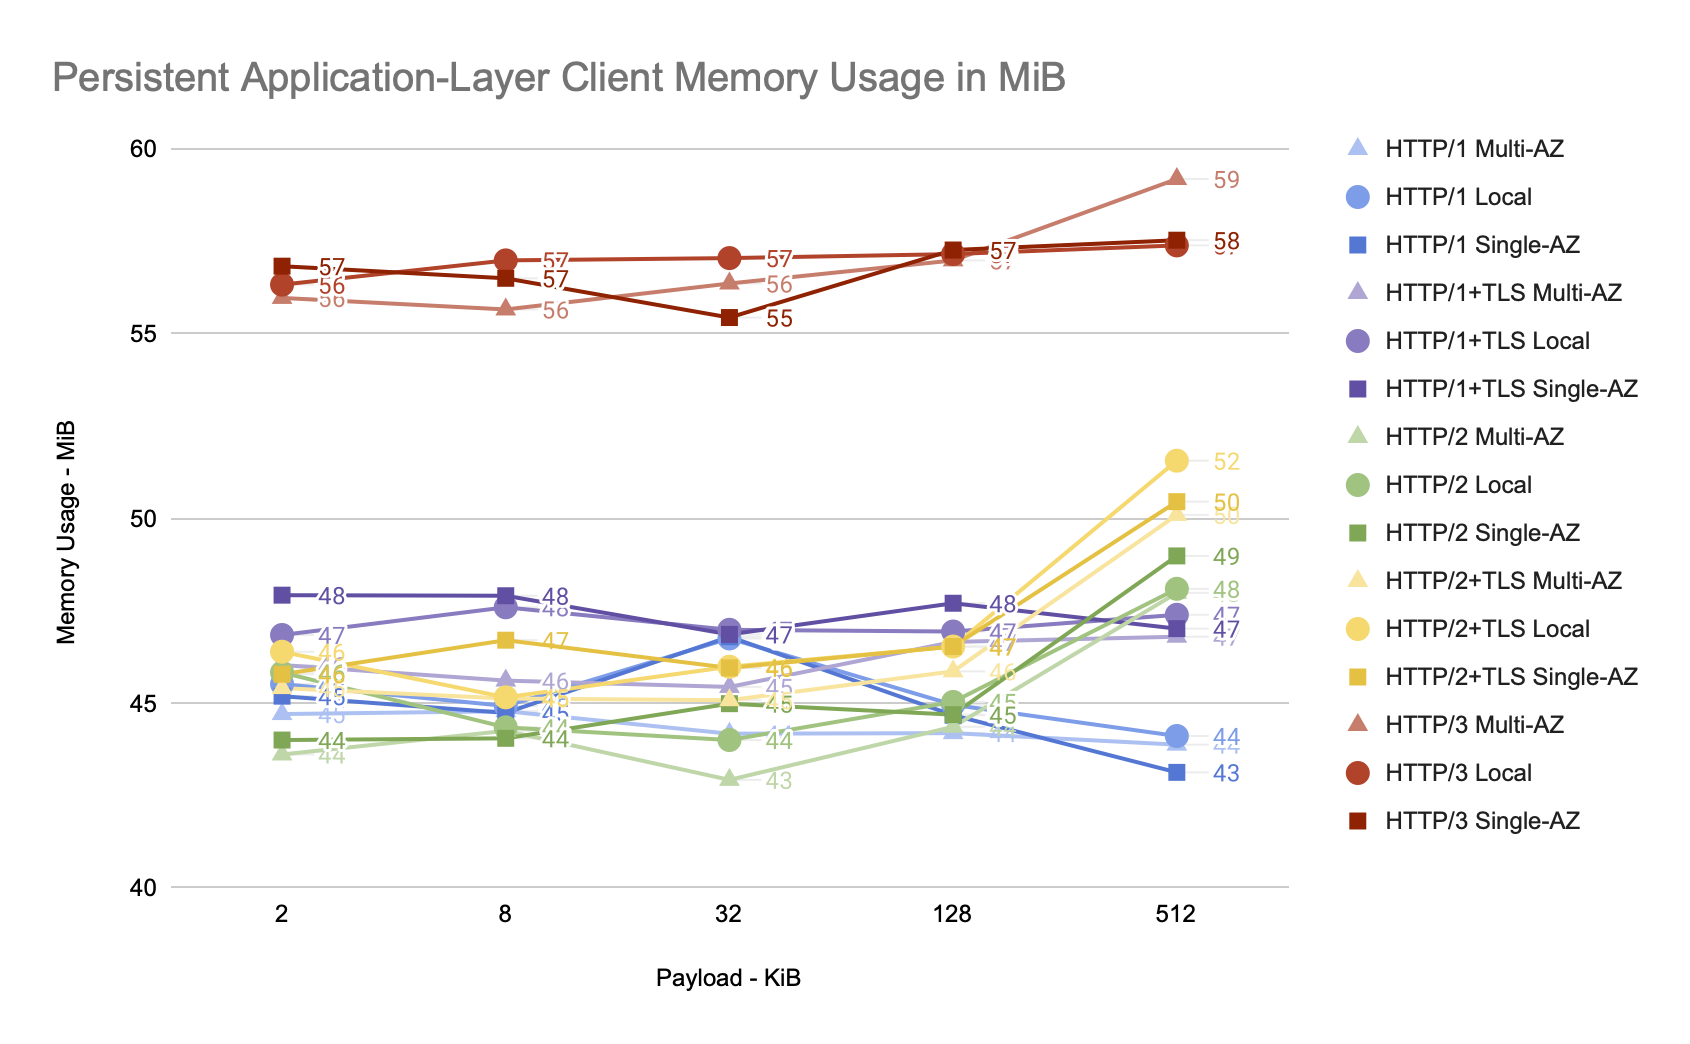
\includegraphics[width=\linewidth]{figures/charts/Persistent Application-Layer Client Memory Usage in MiB.png}
    \caption{Persistent Application-Layer Client Memory Usage in MiB}
    \label{fig:persistent_client_app_memory}
\end{figure}

\begin{figure}[h!]
    \centering
    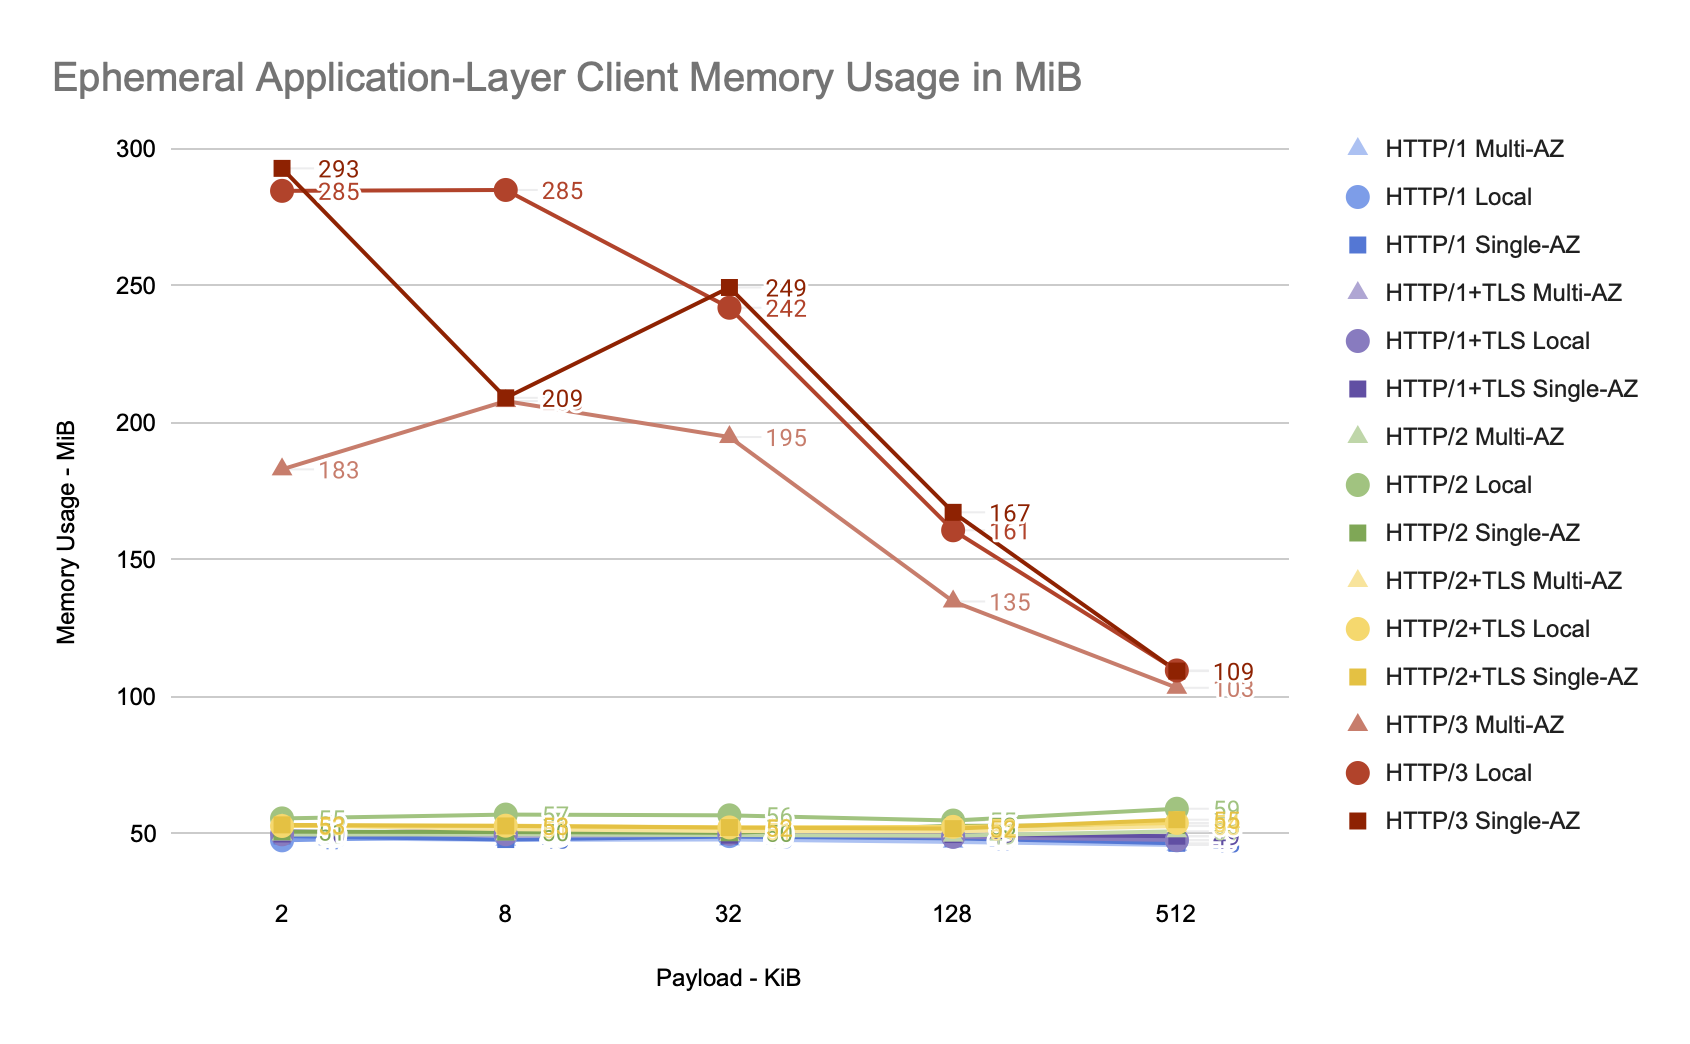
\includegraphics[width=\linewidth]{figures/charts/Ephemeral Application-Layer Client Memory Usage in MiB.png}
    \caption{Ephemeral Application-Layer Client Memory Usage in MiB}
    \label{fig:ephemeral_client_app_memory}
\end{figure}

\begin{figure}[h!]
    \centering
    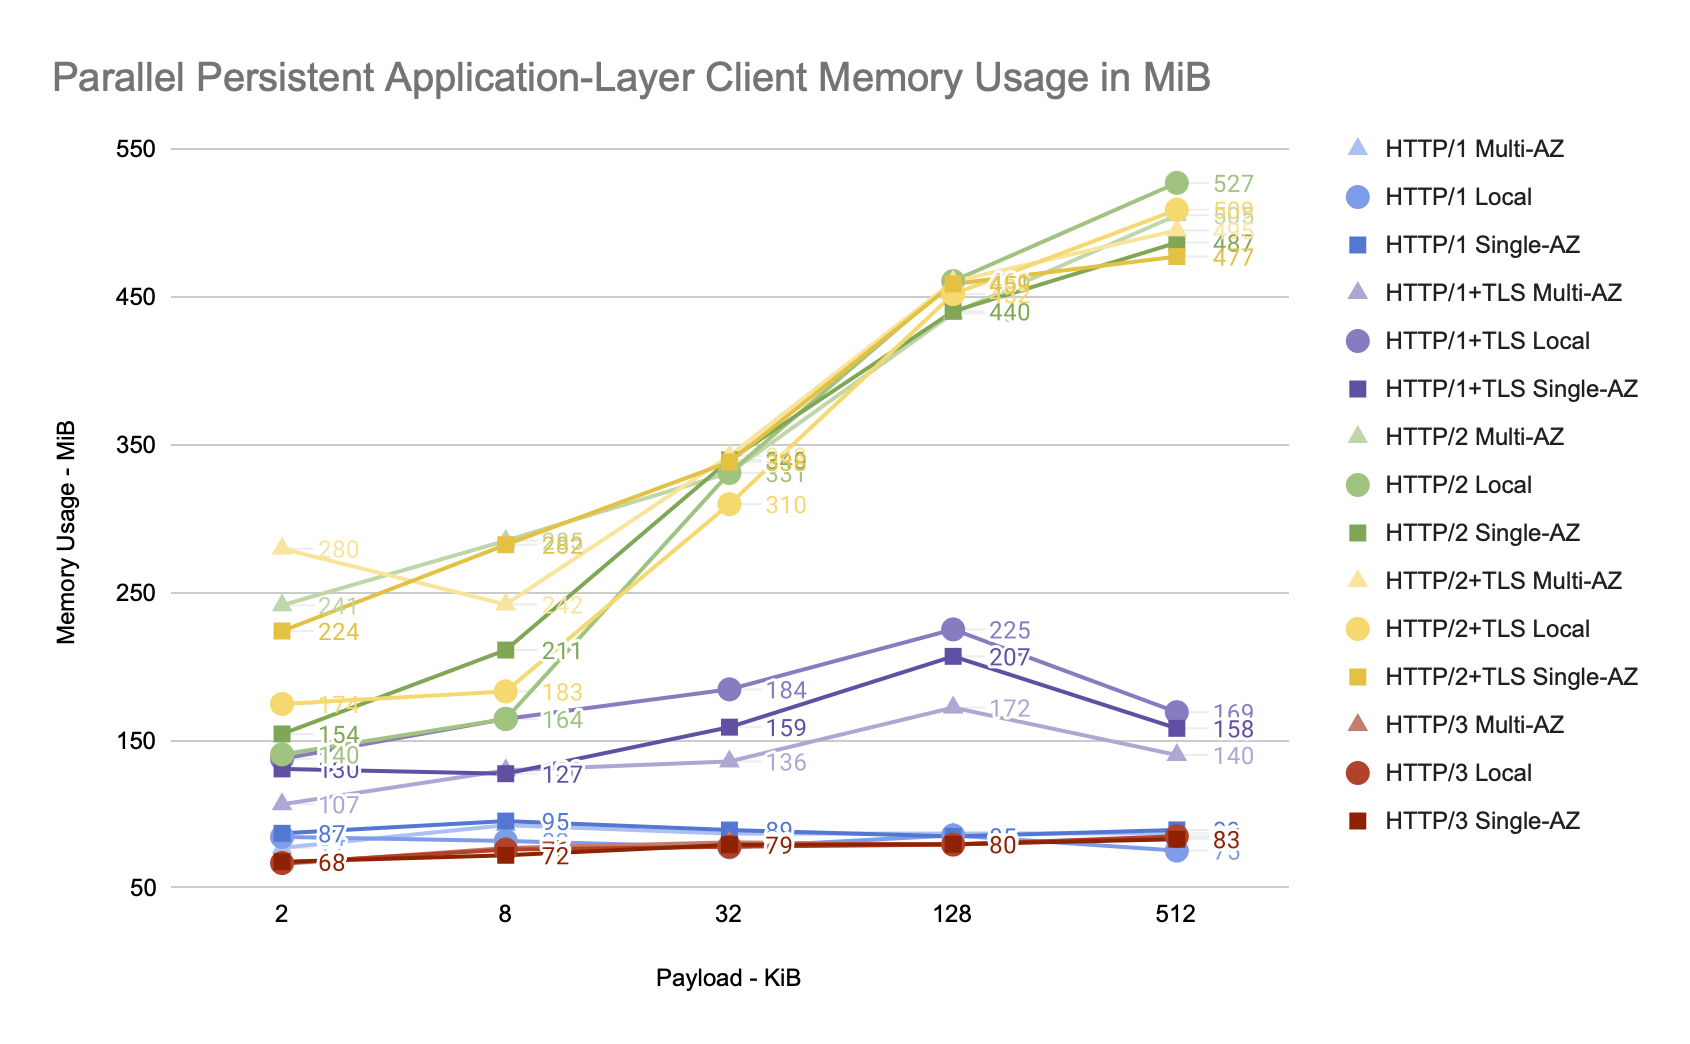
\includegraphics[width=\linewidth]{figures/charts/Parallel Persistent Application-Layer Client Memory Usage in MiB.png}
    \caption{Parallel Persistent Application-Layer Client Memory Usage in MiB}
    \label{fig:parallel_client_app_memory}
\end{figure}

\begin{figure}[h!]
    \centering
    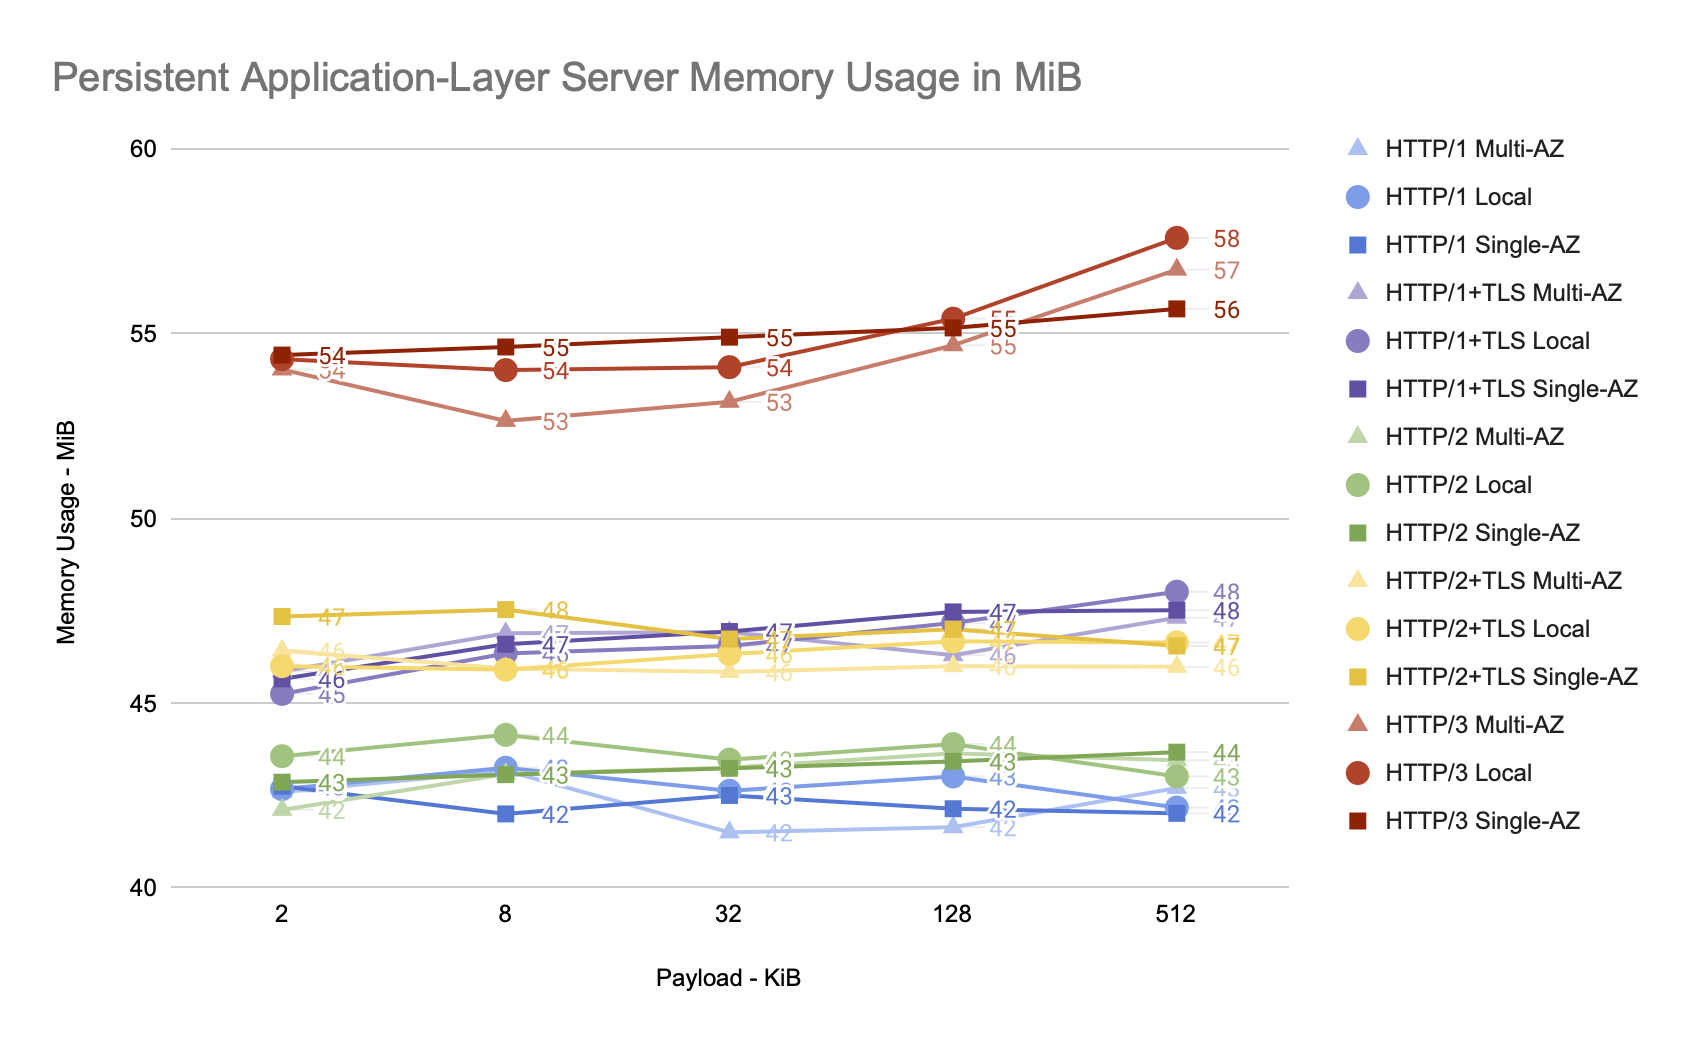
\includegraphics[width=\linewidth]{figures/charts/Persistent Application-Layer Server Memory Usage in MiB.png}
    \caption{Persistent Application-Layer Server Memory Usage in MiB}
    \label{fig:persistent_server_app_memory}
\end{figure}

\begin{figure}[h!]
    \centering
    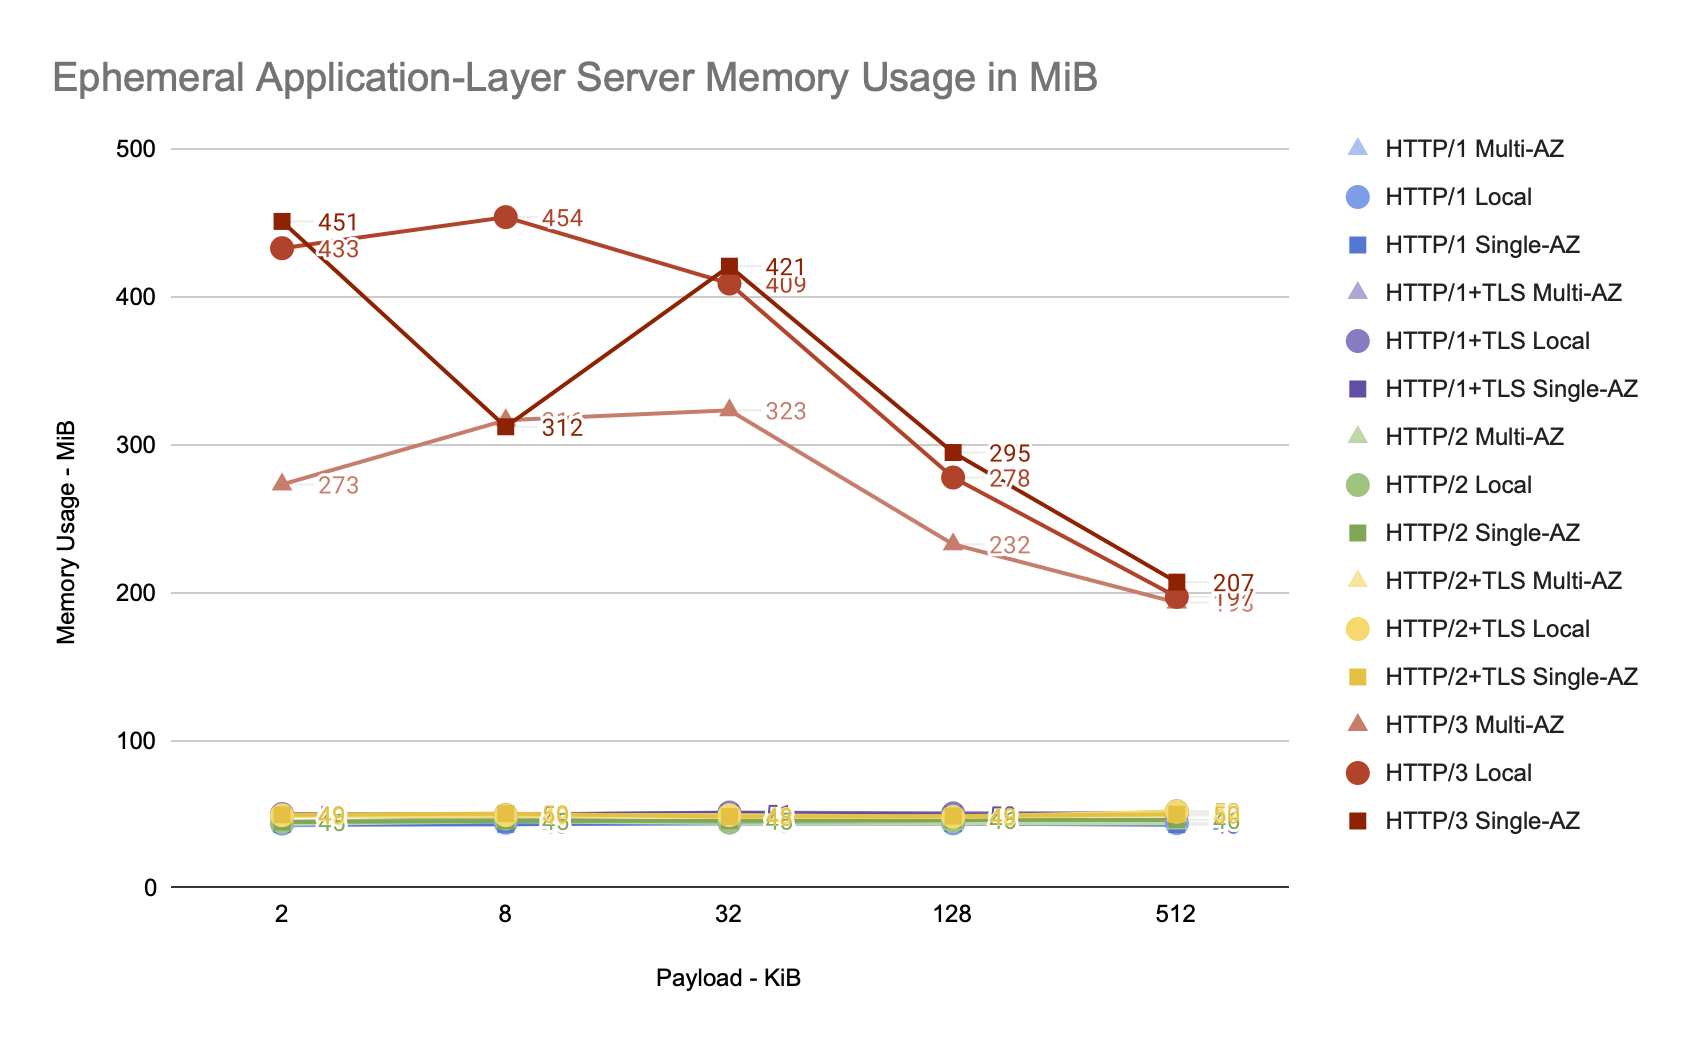
\includegraphics[width=\linewidth]{figures/charts/Ephemeral Application-Layer Server Memory Usage in MiB.png}
    \caption{Ephemeral Application-Layer Server Memory Usage in MiB}
    \label{fig:ephemeral_server_app_memory}
\end{figure}

\begin{figure}[h!]
    \centering
    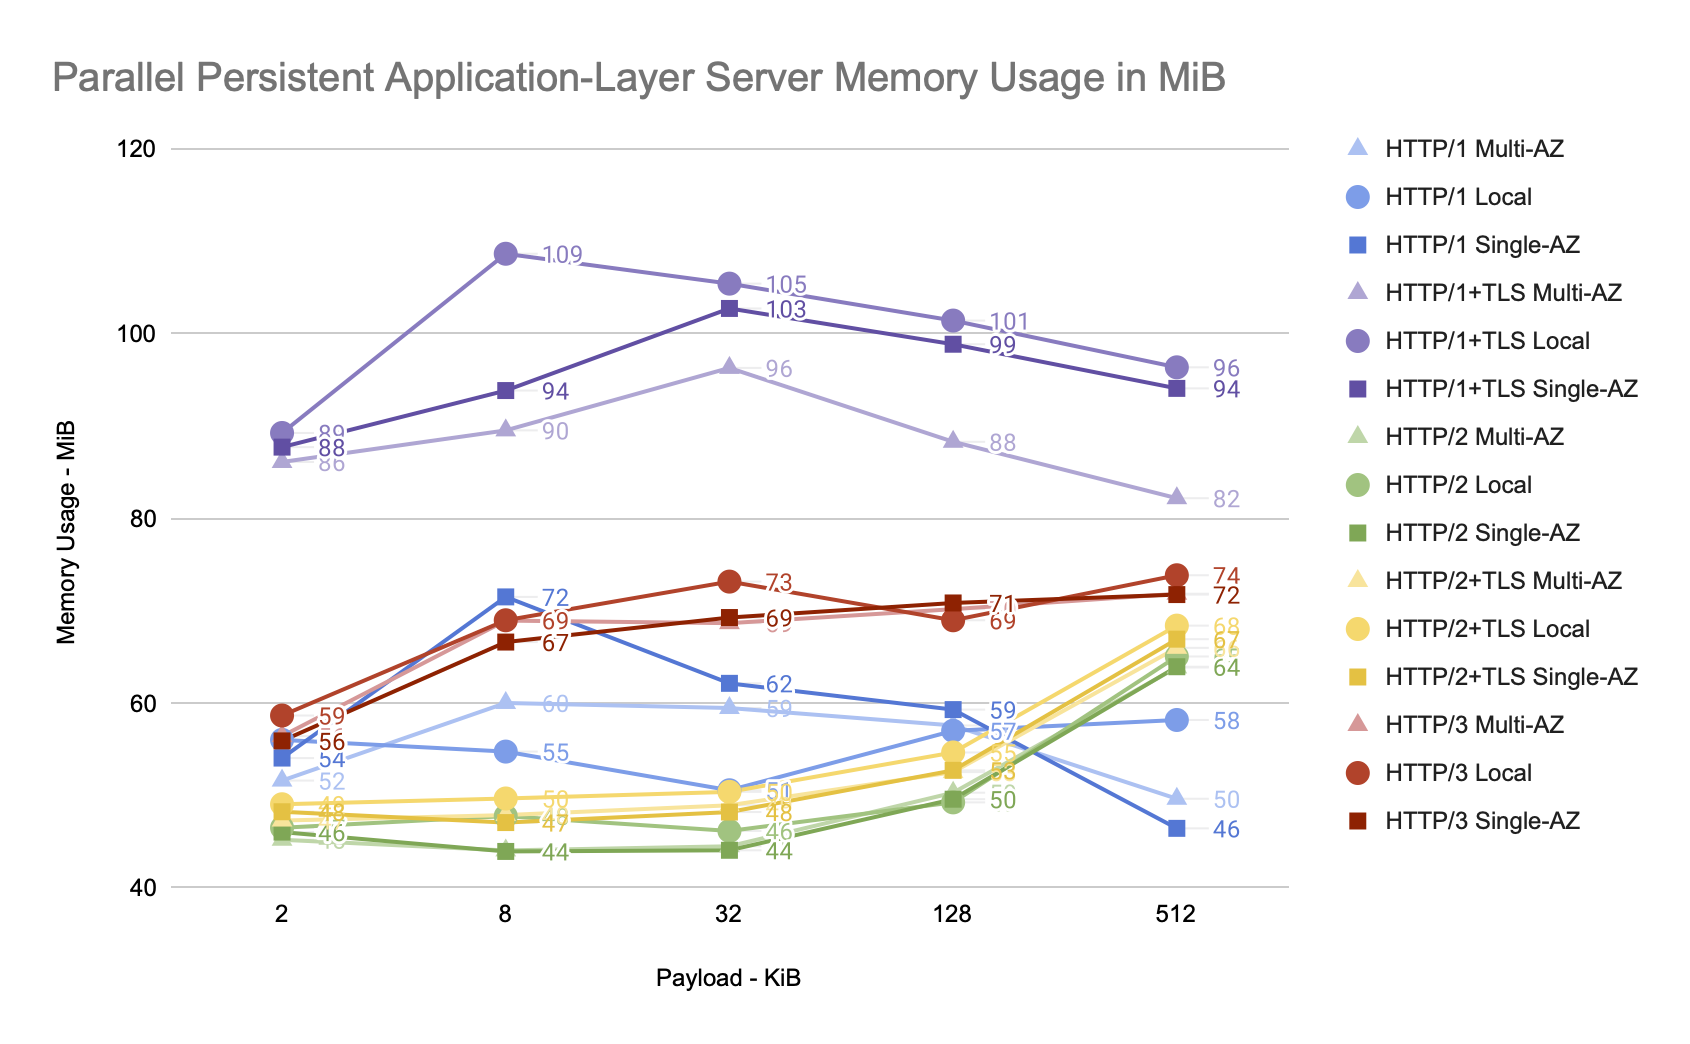
\includegraphics[width=\linewidth]{figures/charts/Parallel Persistent Application-Layer Server Memory Usage in MiB.png}
    \caption{Parallel Persistent Application-Layer Server Memory Usage in MiB}
    \label{fig:parallel_server_app_memory}
\end{figure}

\clearpage
